\documentclass{book}
\usepackage{fancyhdr}
\usepackage{textcomp}
\usepackage{hyperref}
\usepackage{graphicx}
\usepackage{ifthen}
\usepackage{multicol}
\usepackage{makeidx}
\usepackage{mdwlist}
\usepackage[hscale=0.8,twoside]{geometry}
\usepackage[sf,medium,compact]{titlesec}

\makeindex

\newcommand{\importrcp}[2]{\def\ThisFile{#1}\input{#2}}
\newcommand{\half}{\sfrac{1}{2}}
\newcommand{\quarter}{\sfrac{1}{4}}
\newcommand{\threequarter}{\sfrac{3}{4}}
\newcommand{\eighth}{\sfrac{1}{8}}
\newcommand{\third}{\sfrac{1}{3}}
\newcommand{\twothird}{\sfrac{2}{3}}
\newcommand{\Tp}[1]{#1\,tbsp}
\newcommand{\tp}[1]{#1\,tsp}
\newcommand{\C}[1]{#1\,cup}
\newcommand{\oz}[1]{#1\,oz}
\newcommand{\cm}[1]{#1\,cm}
\newcommand{\inch}[1]{#1$^{\prime\prime}$}
\newcommand{\lbs}[1]{#1\,lbs}
\newcommand{\qt}[1]{#1\,qt}
\newcommand{\gr}[1]{#1\,g}
\newcommand{\kgr}[1]{#1\,kg}
\newcommand{\gal}[1]{#1\,gallon}
\newcommand{\ltr}[1]{#1\,L}
\newcommand{\mL}[1]{#1\,mL}
\newcommand{\tF}[1]{#1\,\textdegree{}F}
\newcommand{\tC}[1]{#1\,\textcelsius}
\newcommand{\ang}[1]{#1\,\textdegree}
\newcommand{\UNTESTED}{\textbullet{}}
\newcommand{\FIXME}{\textdaggerdbl{}}
\newcommand{\seerecipe}[1]{\nameref{rcp:#1}~(See page~\pageref{rcp:#1})\ }
\newcommand{\up}[1]{{\thinspace$^{\hbox{\scriptsize#1\fam=-1}}$}}
\newcommand{\pronounce}[1]{(\textsl{#1})}
\newcommand{\method}[1]{This recipe is made using \nameref{method:#1}.\par}

\newenvironment{ingredients}
{\noindent Ingredients:\begin{itemize*}\setlength{\itemindent}{-1.2pc}\renewcommand{\labelitemi}{$\cdot$}}{\end{itemize*}}

\newenvironment{directions}
{\smallskip\begin{enumerate*}}{\end{enumerate*}}

\catcode`\@=11
%    \@car is actually already defined in latex.tex, but for
%    maximum robustness it needs to have the \long prefix:
\long\def\@car#1#2\@nil{#1}
\long\def\@first#1#2{#1}
\long\def\@second#1#2{#2}
\long\def\ifempty#1{\expandafter\ifx\@car#1@\@nil @\@empty
  \expandafter\@first\else\expandafter\@second\fi}
  \catcode`\@=12
  
  \long\def\test#1{\begingroup \toks0{[#1]}%
    \newlinechar`\/\message{/\the\toks0:
      \ifempty{#1}{EMPTY}{NOT empty}%
      }\endgroup}
      
\newcommand{\nonempty}[2]{\ifempty{#1}{}{#2}}

\newenvironment{recipe}[3]{
\newcommand{\theme}[1]{\index{##1!#1}##1}
\newcommand{\stheme}[1]{\index{##1!#1}}
\newcommand{\htheme}[2]{\index{##2!##1!#1}##1 ##2}
\newcommand{\shtheme}[2]{\index{##2!##1!#1}##1}
\newcommand{\hint}[1]{\smallskip \noindent \textsl{##1} \par}
\newcommand{\subrecipe}[1]{\subsection*{##1}}
\newcommand{\slashitem}[1]{\item Slash the top of the loaf. \par\hfil\includegraphics{##1}\hfil\par}
\section{#1}\label{\ThisFile}
\nonempty{#2#3}{
\noindent
	\nonempty{#2}{From #2.}
\hfil 
	\nonempty{#3}{Makes #3.}
\par}
}{\vspace*\fill\pagebreak[2]}
\titlelabel{}
\fancyhf{}
\renewcommand{\chaptermark}[1]{\markboth{#1}{}}
\fancyhf{}
\fancyhead[LE,RO]{\thepage}
\fancyhead[RE]{\textit{\nouppercase{\leftmark}}}
\fancyhead[LO]{}
\widowpenalty=0
\clubpenalty=0


\begin{document}
\titlelabel{}
\pagestyle{fancy}
\fancyhf{}
\renewcommand{\chaptermark}[1]{\markboth{#1}{}}
 
\fancyhf{}
\fancyhead[LE,RO]{\thepage}
\fancyhead[RE]{\textit{\nouppercase{\leftmark}}}
\fancyhead[LO]{}

\thispagestyle{plain}

\title{Laboratory Procedures for Basic Applied Biochemistry \\
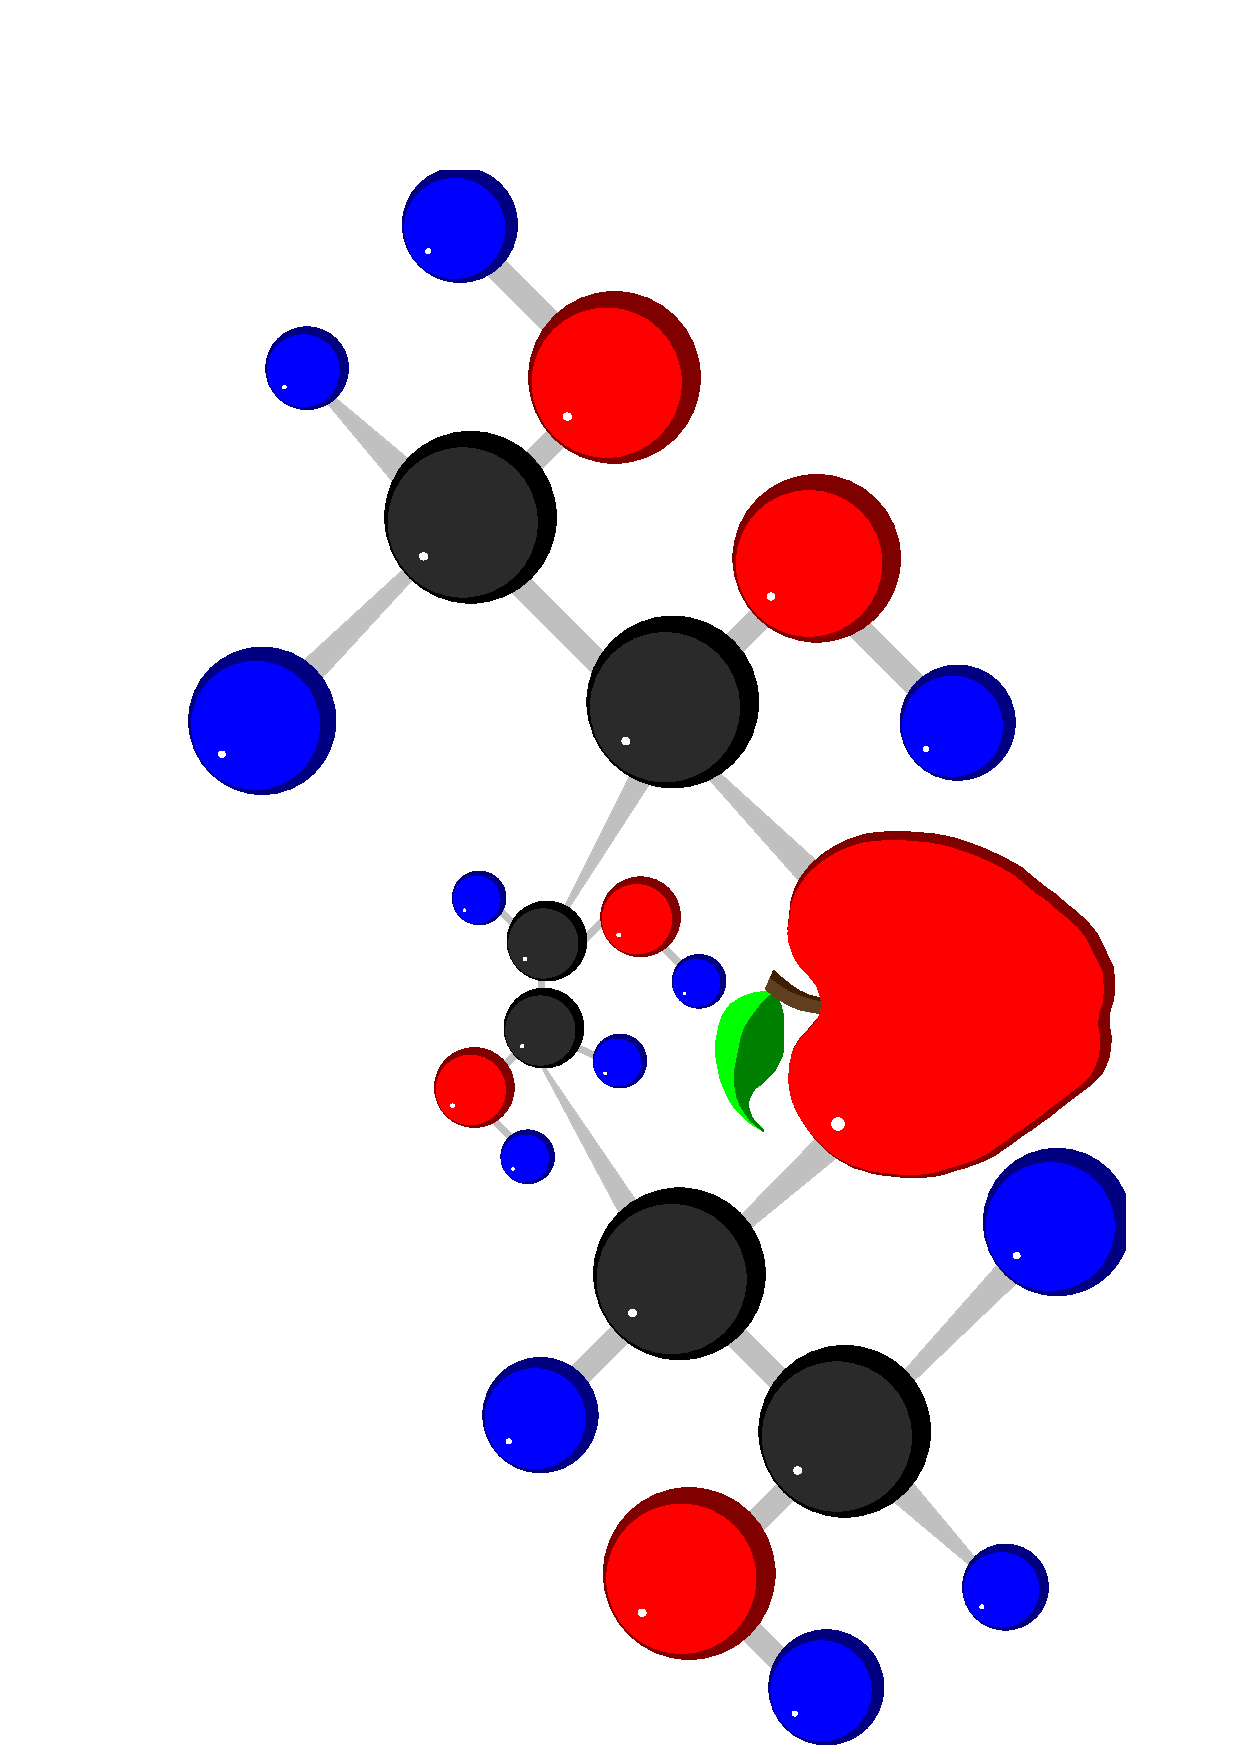
\includegraphics[width=0.5\textwidth,angle=-90]{CoverLogo} 
}
\author{ Andre Masella }
\date{\today{} -- \input{Revision.tex}}
\maketitle

\tableofcontents

\chapter{Introduction}

\section{Welcome}

These are recipes I have collected from various places. Most of them are
family recipies. Some recpies are marked \UNTESTED meaning I have not
made them, but they seem sound.  I will test them eventually. Some recipes are marked with \FIXME{}. These are undoubtedly family recipes lacking quantities. If you make one of these, please accurately measure the ingredients and help me update this book.\par

\section{Preparation}

This has been typeset using \LaTeX{}, using custom recipe environments.
The cover graphic was made in Inkscape.\par

\section{Conversion Hints}

It is good to know that: \par

\begin{tabular}{c c c c c}
\tp{3} & = & \Tp{1} & = & \oz{\half} \\
\C{1} & = & \oz{8} & = & \qt{\quarter}
\end{tabular}

\section{Trivia and Myths}
\begin{itemize}
\item Water in a stainless steel pot should be salted after boiling as the salt will corrode and pit the metal.
\item When removing meat from pasta sauce, a small well of pasta water should be added to ``rinse'' the meat as it is being removed.
\item When dressing pasta the Nonna-way, toss the pasta is half the cheese and tomato sauce, put into individual dishes, sprinkle remaining cheese and ladle reamaining sauce on top. Adding sauce with cheese on top is ``ristorante''-style.
\item If substituting canned tomatoes, diced tomates are equivalent to tomato pieces is most recipes and crushed tomatoes are equivalent to pur\'ee.
\item To raise bread faster, put the bread in a cold oven with a bowl or pot of boiled water. Reheat the water when it cools.
\item To make a firmer crust on breads, increase the oven temperature and steam the oven by cracking the door and wetting the sides of the oven with a spray bottle of water.
\end{itemize}

\section{Bread Cooking}
According to Alton Brown, bread should be cooked until it reaches an internal termperature of \tF{207}. Any higher than \tF{210} or lower than \tF{205} will result in bad bread. Times are suggestions based on experience before cooking by temperature or for recipes where inserting a temperature probe is not practical. Any recipes where bread is not cooked to \tF{207} are explicitly labelled.

\chapter{Dip}


\chapter{Glossary}
\begin{description}
\item[baccal\`a] --- Dried salted cod.
\item[culis\"e] --- The cooking water from pasta.
\item[p\"epparul\"e] --- Sweet red pepper flakes. Subsitute paprika.
\item[squicala] --- The arbirary amount of oil needed by recipes that do not specify a quantity of oil. Approximately 1-\Tp{3}.
\item[window-pane test] --- A test to see if bread is sufficiently kneaded. Strech a small section of bread gently. If the bread can be stretched thin enough for light to pass through with out tearing, the dough is ready.
\end{description}

\printindex

\end{document}
